% !TeX TXS-program:compile = txs:///arara
% arara: pdflatex: {shell: yes, synctex: no, interaction: batchmode}
% arara: pdflatex: {shell: yes, synctex: no, interaction: batchmode} if found('log', '(undefined references|Please rerun|Rerun to get)')

\documentclass[11pt,a4paper]{ltxdoc}
%\usepackage{crimson}
\usepackage{bera}
\usepackage{inconsolata}
%\renewcommand*\ttdefault{cmvtt}
\usepackage[T1]{fontenc}
\usepackage[scale=0.875]{cabin}
\usepackage{euromoney}
\usepackage{fancyvrb}
\usepackage{fancyhdr}
\usepackage{tabularray}
\usepackage{fontawesome5}
\fancyhf{}
\renewcommand{\headrulewidth}{0pt}
\lfoot{\sffamily\small [euromoney]}
\cfoot{\sffamily\small - \thepage{} -}
\rfoot{\hyperlink{matoc}{\small\faArrowAltCircleUp[regular]}}
\usepackage{hologo}
\providecommand\tikzlogo{Ti\textit{k}Z}
\providecommand\TeXLive{\TeX{}Live\xspace}
\let\TikZ\tikzlogo

\usepackage{hyperref}
\urlstyle{same}
\hypersetup{pdfborder=0 0 0}
\usepackage[margin=2cm]{geometry}
\setlength{\parindent}{0pt}
\def\TPversion{0.1.0}
\def\TPdate{06/09/2024}
\usepackage{tcolorbox}
\tcbuselibrary{skins,hooks,listingsutf8}
%\usepackage{soul}
%\sethlcolor{lightgray!25}

\lstset{
	language=[LaTeX]TeX,%
	basicstyle=\ttfamily,%
	keywordstyle={\color{blue}},%
	classoffset=0,%
	keywords={usepackage,\includegraphics,xstring,listofitems,tikz,calc,simplekv,graphicx},%
	alsoletter={-},%
	keywordstyle={\color{blue}},%
	classoffset=1,%
	alsoletter={-},%
	morekeywords={euromoney},%
	keywordstyle={\color{violet}},%
	classoffset=2,%
	alsoletter={-},%
	morekeywords={\BilletsEuro,\PiecesEuro,\EuroBanknotes,\EuroCoins},%
	keywordstyle={\color{green!50!black}},%
	classoffset=3,%
	morekeywords={RefHeight,Style,AutoHeight,OffsetH,OffsetV,Stack,Angle,HauteurRef,HauteurAuto,DecalH,DecalV,Empilage},%
	keywordstyle={\color{orange}}
}

\newtcblisting{DemoCode}[1]{%
	enhanced,width=\linewidth,%
	bicolor,size=title,%
	colback=cyan!10!white,%
	colbacklower=cyan!5!white,%
	colframe=cyan!75!black,%
	listing options={%
		breaklines=true,%
		breakatwhitespace=true,%
		style=tcblatex,basicstyle=\small\ttfamily,%
		tabsize=4,%
		commentstyle={\itshape\color{gray}},
		keywordstyle={\color{blue}},%
		classoffset=0,%
		keywords={usepackage,\includegraphics,xstring,listofitems,tikz,calc,simplekv,graphicx},%
		alsoletter={-},%
		keywordstyle={\color{blue}},%
		classoffset=1,%
		alsoletter={-},%
		morekeywords={euromoney},%
		keywordstyle={\color{violet}},%
		classoffset=2,%
		alsoletter={-},%
		morekeywords={\BilletsEuro,\PiecesEuro,\EuroBanknotes,\EuroCoins},%
		keywordstyle={\color{green!50!black}},%
		classoffset=3,%
		morekeywords={RefHeight,Style,AutoHeight,OffsetH,OffsetV,Stack,Angle,HauteurRef,HauteurAuto,DecalH,DecalV,Empilage,height},%
		keywordstyle={\color{orange}}
	},%
	#1
}
\NewDocumentCommand\MontreCode{ m }{%
	\lstinline{#1}%
}

\begin{document}

\thispagestyle{empty}

\begin{center}
	\begin{minipage}{0.88\linewidth}
		\begin{tcolorbox}[colframe=yellow,colback=yellow!15]
			\begin{center}
				\begin{tabular}{c}
					{\Huge \texttt{euromoney}}\\
					\\
					{\LARGE Insert 'vectorial' coins or} \\
					{\LARGE banknotes in euro.} \\
					\\
					{\small \texttt{Version \TPversion{} -- \TPdate}}
				\end{tabular}
			\end{center}
		\end{tcolorbox}
	\end{minipage}
\end{center}

\begin{center}
	\begin{tabular}{c}
		\texttt{Cédric Pierquet}\\
		{\ttfamily c pierquet -- at -- outlook . fr}\\
		\texttt{\url{https://github.com/cpierquet/euromoney}} \\
	\end{tabular}
\end{center}

\hrule

\vfill

\begin{tcolorbox}[colframe=lightgray,colback=lightgray!5]
	\begin{center}
		\PiecesEuro[HauteurRef=1cm,Style=full,HauteurAuto]{4*2+3*1+4*0.2+1*0.1+2*0.01}
		
		\vspace*{2.5mm}
		
		\PiecesEuro[Empilage=V,HauteurRef=3cm,HauteurAuto]{4*2+3*1+4*0.2+1*0.1+2*0.01}
		
		\vspace*{2.5mm}
		
		\BilletsEuro[Style=nb,HauteurRef=1.75cm,DecalV=0.5cm,HauteurAuto]{4*100+2*50+20+4*10+3*5}
		
		\vspace*{2.5mm}
		
		\BilletsEuro[Style=full,HauteurAuto]{100+50+20+5}
	\end{center}
\end{tcolorbox}

\vfill~

\hrule

\medskip

\emph{%
	The pdf files were obtained by converting vector \texttt{svg} (public domain) files from the \href{https://openclipart.org/artist/frankes?p=3}{\texttt{openclipart}} database, and in particular from files supplied by \href{https://openclipart.org/artist/frankes?p=3}{\texttt{frankes}}.
}

\medskip

\hrule

\vspace*{5mm}

\pagebreak

\phantomsection

\hypertarget{matoc}{}

\tableofcontents

\vspace*{5mm}

%\hrule

\pagebreak

\section{Introduction}

\subsection{Description, loading}

The idea is to propose macros to insert coins and banknotes in euro.

\begin{DemoCode}{listing only}
\usepackage{euromoney}
\end{DemoCode}

The \MontreCode{euromoney} package loads :

\begin{itemize}
	\item \lstinline{xstring} ;
	\item \lstinline{simplekv} ;
	\item \lstinline{graphicx} ;
	\item \lstinline{tikz} with \MontreCode{calc} library ;
	\item \lstinline{listofitems}.
\end{itemize}

\subsection{Features}

It's possible to present multiple coins or multiples banknotes :

\begin{itemize}
	\item with global height ;
	\item with height automatically adjusted (compared to 2€ coin and 500€ banknote) ;
	\item with stacking.
\end{itemize}

\section{Global names, samples}

\subsection{Global names}

Each coin or bill is a vectorial pdf and there's three styles :

\begin{itemize}
	\item \MontreCode{full} colored version ;
	\item \MontreCode{simple} colored version with \MontreCode{simple} suffix ;
	\item \MontreCode{bw} version with \MontreCode{simplebw} suffix .
\end{itemize}

Available basenames are :

\begin{itemize}
	\item \texttt{500euro} ; \texttt{200euro} ; \texttt{100euro} ; \texttt{50euro} ; \texttt{20euro} ; \texttt{10euro} and \texttt{5euro} ;
	\item \texttt{2euro} ; \texttt{1euro} ; \texttt{50cent} ; \texttt{20cent} ; \texttt{10cent} ; \texttt{5cent} ; \texttt{2cent} and \texttt{1cent}.
\end{itemize}

\begin{DemoCode}{}
%manual insertion
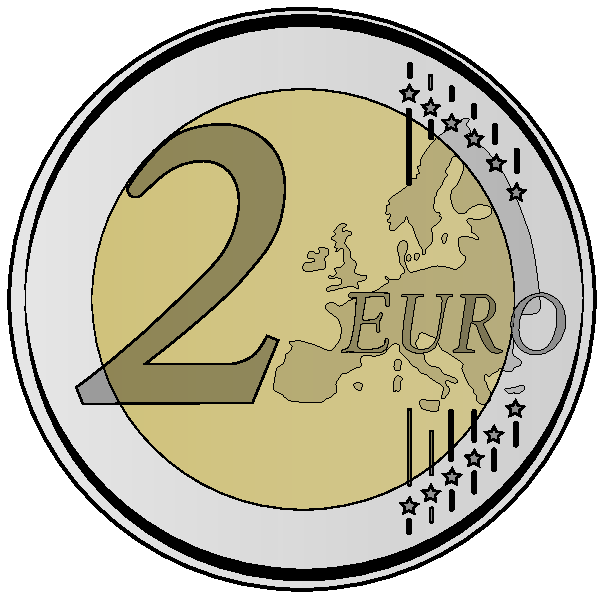
\includegraphics[height=25.75mm]{2euro}%         w/o suffix

\includegraphics[height=25.75mm]{2eurosimple}%   with simple suffix

\includegraphics[height=25.75mm]{2eurosimplebw}% with simplebw suffix
\end{DemoCode}

\subsection{Size of graphics}

Banknotes of \MontreCode{Style=full} are bigger than other styles, so the output doc can be bigger size.

For example, 100€ banknote's size is 933~Ko.

\section{Macro for coins}

\subsection{Usage}

The coins macro is :

\begin{DemoCode}{listing only}
\EuroCoins[keys]{list of coins}
\end{DemoCode}

Available keys are :

\begin{itemize}
	\item \MontreCode{RefHeight} := height (default \MontreCode{2cm}) for the coins (relative to 2€ if \MontreCode{AutoHeight=true}) ;
	\item \MontreCode{Style} := style for coins (default \MontreCode{simple}), within \MontreCode{full/simple/bw} ;
	\item \MontreCode{AutoHeight} := boolean (default \MontreCode{false}) for adjusting heights of coins ;
	\item \MontreCode{OffsetH} := horizontal offset (default \MontreCode{0pt}) for multiple coins (side by side if \MontreCode{0pt}) ;
	\item \MontreCode{OffsetV} := vertical offset (default \MontreCode{5mm}) for multiple coins vertically stacked ;
	\item \MontreCode{Stack} := sens of stacking (default \MontreCode{H}) for mutiple coins.
\end{itemize}

List of coins can be given within \MontreCode{3*2+4*1+2*0.2+4*0.1} for example.

\subsection{Examples}

\begin{DemoCode}{}
%sample with one coin
\EuroCoins{2}\EuroCoins{1}\EuroCoins{0.5}\EuroCoins{0.2}%
\EuroCoins{0.1}\EuroCoins{0.05}\EuroCoins{0.02}\EuroCoins{0.01}
\end{DemoCode}

\begin{DemoCode}{}
%multiple coins, side by side, global height
\EuroCoins{2+1+0.5+0.2+0.1+0.05+0.02+0.01}
\end{DemoCode}

\begin{DemoCode}{}
%stacked coins (b&w), horizontally with correct scaling
\EuroCoins[RefHeight=3cm,AutoHeight,OffsetH=7.5mm,Style=bw]{4*2+3*1+4*0.2+1*0.1+2*0.01}
\end{DemoCode}

\begin{DemoCode}{}
%stacked coins (full resolution), vertically with correct scaling
\EuroCoins[Stack=V,RefHeight=3cm,AutoHeight,Style=full]{4*2+3*1+4*0.2+1*0.1+2*0.01}
\end{DemoCode}

\section{Macro for banknotes}

\subsection{Usage}

The banknotes macro is :

\begin{DemoCode}{listing only}
\EuroBanknotes[keys]{list of banknotes}
\end{DemoCode}

Stacking is globally set, and available keys are :

\begin{itemize}
	\item \MontreCode{RefHeight} := height (default \MontreCode{2cm}) for the banknotes (relative to 500€ if \MontreCode{AutoHeight=true}) ;
	\item \MontreCode{Style} := style for banknotes (default \MontreCode{simple}), within \MontreCode{full/simple/bw} ;
	\item \MontreCode{AutoHeight} := boolean (default \MontreCode{false}) for adjusting heights of banknotes ;
	\item \MontreCode{OffsetH} := horizontal offset (default \MontreCode{0pt}) for multiple banknotes (side by side if \MontreCode{0pt}) ;
	\item \MontreCode{OffsetV} := vertical offset (default \MontreCode{5mm}) for multiple banknotes vertically stacked ;
	\item \MontreCode{Stack} := type of stacking (default \MontreCode{H}) within \MontreCode{H/fan} ;
	\item \MontreCode{Angle} := rotation (default \MontreCode{10}) for \texttt{fan} stacking.
\end{itemize}

List of banknotes, for \texttt{H} stacking, can be given within \MontreCode{2*100+3*50+10+5} for example.

List of banknotes, for \texttt{fan} stacking, can be given within \MontreCode{5+5+10+10+20+50+100+200+200} for example.

\subsection{Examples}

\begin{DemoCode}{}
%sample with one banknote
\EuroBanknotes{500}\EuroBanknotes{200}\EuroBanknotes{100}\EuroBanknotes{50}\\
\EuroBanknotes{20}\EuroBanknotes{10}\EuroBanknotes{5}
\end{DemoCode}

\begin{DemoCode}{}
%multiple banknotes, side by side, global height
\EuroBanknotes{50+20+5}
\end{DemoCode}

\begin{DemoCode}{}
%multiple banknotes, side by side, with correct scaling
\EuroBanknotes[RefHeight=3cm,Style=full,AutoHeight]{100+10+5}
\end{DemoCode}

\begin{DemoCode}{}
%stacked banknotes (b&w), with correct scaling
\EuroBanknotes[OffsetH=7.5mm,Style=bw,AutoHeight]{4*100+2*50+20+4*10+3*5}
\end{DemoCode}

\begin{DemoCode}{}
%syde by side banknotes, with correct scaling
\EuroBanknotes[RefHeight=1.75cm,AutoHeight]{4*100+2*50+20+4*10+3*5}
\end{DemoCode}

\begin{DemoCode}{}
%fan stacking, with adjusted offsets
\EuroBanknotes%
  [Stack=fan,RefHeight=2.05cm,AutoHeight,Angle=17.5,%
  OffsetH=0.1mm,OffsetV=0mm]%
  {5+5+10+10+20+50+100+200+200}
\end{DemoCode}

\pagebreak

\section{French version}

Il est possible d'utiliser les commandes en version francisée :

\begin{DemoCode}{listing only}
\PiecesEuro[clés]{liste de pièces}
\BilletsEuro[clés]{liste de billets}
\end{DemoCode}

Les clés disponibles sont :

\begin{itemize}
	\item \MontreCode{HauteurRef} := hauteur (défaut \MontreCode{2cm}) pour les pièces/billets (relativement à celle de 2€ et celui de 500€ si \MontreCode{HauteurAuto=true}) ;
	\item \MontreCode{Style} := style pour les pièces/billets (défaut \MontreCode{simple}), parmi \MontreCode{full/simple/nb} ;
	\item \MontreCode{HauteurAuto} := booléen (défaut \MontreCode{false}) pour adapter les hauteurs ;
	\item \MontreCode{DecalH} := décalage horizontal (défaut \MontreCode{0pt}) pour des empilages (côte à côte si \MontreCode{0pt}) ;
	\item \MontreCode{DecalV} := décalage vertical (défaut \MontreCode{5mm}) pour les empilages verticaux ;
	\item \MontreCode{Empilage} := sens de l'empilage (défaut \MontreCode{H}) éventuel, parmi \MontreCode{H/eventail} suivant le type d'objets.
\end{itemize}

La liste peut être donnée sous la forme \MontreCode{3*2+4*1+2*0.2+4*0.1} pour des affichages \textit{classiques} par exemple.

Pour le cas de billets en éventail, la liste pourra être donnée sous la forme \MontreCode{5+5+10+10+20+50+100+200+200} par exemple.

\begin{DemoCode}{}
%exemple avec une pièce
\PiecesEuro{2}\PiecesEuro{1}\PiecesEuro{0.5}\PiecesEuro{0.2}%
\PiecesEuro{0.1}\PiecesEuro{0.05}\PiecesEuro{0.02}\PiecesEuro{0.01}
\end{DemoCode}

\begin{DemoCode}{}
%pièces multiples, côte à côte, taille uniforme
\PiecesEuro{2+1+0.5+0.2+0.1+0.05+0.02+0.01}
\end{DemoCode}

\begin{DemoCode}{}
%pièces empilées (n&b) horizontalement et tailles ajustées
\PiecesEuro%
  [HauteurRef=3cm,HauteurAuto,DecalH=7.5mm,Style=nb]{4*2+3*1+4*0.2+1*0.1+2*0.01}
\end{DemoCode}

\begin{DemoCode}{}
%pièces empilées (full résolution) verticalement et tailles ajustées
\PiecesEuro%
  [Empilage=V,HauteurRef=3cm,HauteurAuto,Style=full]{4*2+3*1+4*0.2+1*0.1+2*0.01}
\end{DemoCode}

\begin{DemoCode}{}
%exemple avec un billet
\BilletsEuro{500}\BilletsEuro{200}\BilletsEuro{100}\BilletsEuro{50}\\
\BilletsEuro{20}\BilletsEuro{10}\BilletsEuro{5}
\end{DemoCode}

\begin{DemoCode}{}
%plusieurs billets, côte à côte, taille uniforme
\BilletsEuro{50+20+5}
\end{DemoCode}

\begin{DemoCode}{}
%plusieurs billets (full résolution), côte à côte, tailles adaptées
\BilletsEuro[HauteurRef=3cm,Style=full,HauteurAuto]{100+10+5}
\end{DemoCode}

\begin{DemoCode}{}
%billets empilés (n&b), tailles adaptées
\BilletsEuro[DecalH=7.5mm,Style=nb]{4*100+2*50+20+4*10+3*5}
\end{DemoCode}

\begin{DemoCode}{}
%billets côte à côte, tailles adaptées
\BilletsEuro[HauteurRef=1.75cm,HauteurAuto]{4*100+2*50+20+4*10+3*5}
\end{DemoCode}

\begin{DemoCode}{}
%billets en éventail, hauteur et décalages ajustés
\BilletsEuro%
  [Empilage=eventail,HauteurRef=2.05cm,HauteurAuto,Angle=17.5,%
  DecalH=0.1mm,DecalV=0mm]%
  {5+5+10+10+20+50+100+200+200}
\end{DemoCode}

\pagebreak


\section{History}

\begin{quote}
\begin{verbatim}
0.1.0 : Initial version
\end{verbatim}
\end{quote}

\end{document}